	\PassOptionsToPackage{brazil,american}{babel}
\documentclass[12pt]{article}

\usepackage{sbc-template}
\usepackage[brazil,american]{babel}
\usepackage[utf8]{inputenc}

\usepackage{graphicx}
\usepackage{url}
\usepackage{float}
\usepackage{listings}	
\usepackage{color}
\usepackage{todonotes}
\usepackage{algorithmic}
\usepackage{algorithm}
\usepackage{hyperref}

\sloppy

\title{Experimento 9\\ 
	FLIP-FLOPS:"T" E "D"}

\author{
	Lucas Mafra Chagas, 12/0126443 \\
	Marcelo Giordano Martins Costa de Oliveira,  12/0037301
}


\address{Dep. Ciência da Computação -- Universidade de Brasília (UnB)\\
	CiC 116351 - Circuistos Digitais - Turma C
	\email{\{giordano.marcelo, chagas.lucas.mafra\}@gmail.com}
}

\begin{document} 

\maketitle

 \begin{abstract}
	 In this experiment, we will study some types of flip-flops T and D by implementing, verifying their truth tables and comparing with the theoretical well-known results.
 \end{abstract}
     
 \begin{resumo} 
	 Neste experimento, serão estudados os alguns tipos de flip-flops T e D, através de sua implementação e posterior verificação de suas respectivas tabelas verdade, comparando-as com os resultados esperados teoricamente.
 \end{resumo}


\section{Objetivos}
\label{sec:Objetivos}

Descrição e implementação de flip-flops “T” e “D” usando portas lógicas ou flip-flops JK. Construção de flip-flops D gatilhado por nível ou pela borda usando portas lógicas; análise na transição de subida e descida do pulso de relógio. Aplicação dos flip-flops no projeto de um detector de sentido de movimento de um veículo.

\section{Materiais} 
\label{sec:Materiais}

\begin{itemize}
    \item Painel Digital
    
    \item \textit{protoboard}
    
    \item Fios
    
    \item Portas NAND, NOR, NOT, 2xFLIP-FLOP “D” (7474).
    
\end{itemize}


\section{Introdução}
\label{sec:Introducao}

O flip-flop T é um tipo de flip-flop que possui apenas uma entrada: a entrada de toggle T. Sempre que mudamos o estado de T, temos que a saída sofrerá modificação e irá para o seu estado inverso. Quando T possui um valor baixo, a saída permanece com o valor que possuia antes. Quando T possui um valor alto, a saída passa a ser o inverso do que era anteriormente. Temos, portanto, que a tabela verdade deste circuito é da seguinte forma: 

\begin{figure}[H]
	\centering
	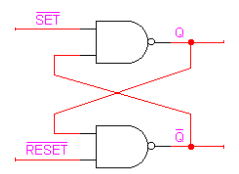
\includegraphics[width=.5\textwidth]{latchRS.png}
	\caption{Latch RS}
	\label{fig:latRS}
\end{figure}

Vemos no circuito que as mudanças de estado de S e R se propagam por 3 portas até chegar nas saídas. Portanto, temos que T precisa ter um pulso de no mínimo 20ns para que a reversão de estado no flip-flop seja garantida. Portanto, temos que a entrada T precisa entrar no circuito conectada à seguinte estrutura:

\begin{figure}[H]
	\centering
	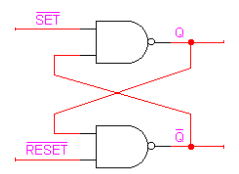
\includegraphics[width=.5\textwidth]{latchRS.png}
	\caption{Latch RS}
	\label{fig:latRS}
\end{figure}

Dessa forma evitamos o estado de indeterminação e o flip-flop funcionará corretamente.
O flip-flop D é um flip-flop que possui uma entrada e um Clock. Essa entrada é diretamente ligada à saída. Portanto, quando mudamos o Clock, independentemente do valor atual que a saída possui, ela irá se ajustar para corresponder ao valor de D. Para este flip-flop, temos que a informação é incluída na saída um ciclo depois de ela ter chegado na entrada.
Fazendo a comparação deste flip-flop com um flip-flop RS gatilhado, temos que este flip-flop nunca terá a mesma entrada para SET e RESET, pois temos que SET recebe D e RESET recebe D. As figuras abaixo ilustram o circuito e o funcionamento deste flip-flop:

\begin{figure}[H]
	\centering
	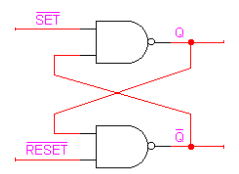
\includegraphics[width=.5\textwidth]{latchRS.png}
	\caption{Latch RS}
	\label{fig:latRS}
\end{figure}


Temos que este flip-flop D tem sua saída modificada apenas quando o Clock é 1. Porém, é possível construir um flip-flop D gatilhado pela borda que permite que a entrada seja modificada ainda quando há a mudança de pulso, de 0 para 1. A imagem abaixo apresenta as características deste flip-flop:


\begin{figure}[H]
	\centering
	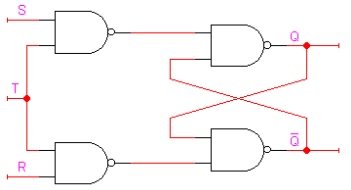
\includegraphics[width=.5\textwidth]{RSgat.png}
	\caption{Latch RS Gatilhado}
	\label{fig:RSgat}
\end{figure}

Este flip-flop é gatilhado pela borda positiva, porém, é possível construir um flip-flop gatilhado pela borda negativa, onde a mudança de estado irá ocorrer quando o pulso vai de 1 para 0.
É possível construir um todos os flip-flops mencionados acima a partir de um flip-flop JK. Para transformar um flip-flop JK em um flip-flop RS apenas conectamos S a J e R a K. Porém, teremos que evitar, para este caso, o estado 11. Para transformar um flip-flop JK em um flip-flop D, é necessário apenas incluir um inversor entre os terminais J e K. Para transformá-lo em um flip-flop T, considera-se que as entradas J e K são ambas T De tal forma, T irá definir se aceita ou não o pulso enviado pelo relógio.
Ao lidar com flip-flops é necessário sempre considerar uma propriedade importante: o tempo de setup do flip-flop. O tempo de setup de um flip-flop é definido como o menor intervalo de tempo em que o sinal da(s) entrada(s) deve(m) estar já no nível correto e ser(em) mantido(s) antes da ocorrência de uma transição no relógio.  Para a família TTL esse tempo é de 20ns.

\section{Procedimentos}
\label{sec:Procedimentos}

Neste experimento, faremos a construção dos flip-flops mencionados acima e analisaremos o seu funcionamento.

\subsection{Montar um flip-flop “T” utilizando apenas portas NAND.}
\label{2.1}

\begin{table}[H]
	\centering
	\begin{tabular}{|c|c|c|c|}
		\cline{1-4}
		\caption{Tabela-Verdade do Latch RS}
		\multicolumn{1}{|c|}{S} & \multicolumn{1}{|c|}{R} & \multicolumn{1}{|c|}{Q} & \multicolumn{1}{|c|}{$\overline{Q}$} \\
		\hline
		1 & 0 & 1 & 0  \\
		\hline
		1 & 1 & 0 & 0 \\
		\hline
		0 & 1 & 0 & 1  \\
		\hline
		1 & 1 & 0 & 0  \\
		\hline
		0 & 0 & 0 & 1  \\
		\hline
		1 & 1 & 0 & 0  \\
		\hline
	\end{tabular}
	
\end{table} 

\subsection{Montar um flip-flop “D” gatilhado por nível.}
\label{2.2}

\href{https://youtu.be/azJt3y337BE}{Vídeo 2.2}

\subsection{Montar um flip-flop “D” gatilhado pela borda.}
\label{2.3}

\href{https://youtu.be/1GDHpbQ8CnU}{Vídeo 2.3}

\subsection{Montar, verificar e explicar o funcionamento de um flip-flop “D” com circuito auxiliar de produção de pulsos.}
\label{2.4}

\href{https://youtu.be/c2MW7RQl_7s}{Vídeo 2.4}

\subsection{Projetar um circuito seqüencial que detecta o sentido de movimento de veículos em uma rua. }
\label{2.5}



\section{Análise dos Resultados}
\label{sec:Resultados}

Faça uma análise crítica dos resultados obtidos nos experimentos. Esta análise pode ser feita item a item ou de uma forma geral.

Dica: Use pesquisa na Internet para tirar as dúvidas sobre edição em \LaTeX .

\section{Conclusão}
\label{sec:Conclusao}

Neste experimento foi possível perceber a importância de um flip-flop na utilização de armazenamento de informações. Vimos que, se construídos corretamente, os flip-flops podem ser úteis em diversas aplicações

\newpage 
% Colocar aqui apenas as respostas dos itens da Auto-Avaliação
\section*{Auto-Avaliação}

\begin{enumerate}
    \item B
    \item C
    \item A
    \item C
    \item C
    \item A
    \item A
    \item A
    \item C
    \item C
\end{enumerate}


\end{document}
